\documentclass[12pt,a4paper,oneside,openany]{book}

% Compilar con pdfLaTeX + BibTeX; véase README.md.
\usepackage[utf8]{inputenc}
\usepackage[T1]{fontenc}
\usepackage[spanish,es-nodecimaldot]{babel}
\usepackage{lmodern}
\usepackage{microtype}
\usepackage[a4paper,margin=3cm]{geometry}
\usepackage{booktabs}
\usepackage{graphicx}
\usepackage{tabularx}
\usepackage{array}
\usepackage{natbib}
\usepackage{hyperref}

\hypersetup{
  hidelinks,
  hypertexnames=false,
  pdftitle={Diseño y evaluación de un marco de trabajo basado en agentes para la búsqueda de soluciones en tareas de detección y spoiling de clickbait},
  pdfauthor={Miguelángel Díaz Cerecetto}
}
\setlength{\parindent}{1.2em}
\setlength{\parskip}{0.25em}
\newcolumntype{Y}{>{\raggedright\arraybackslash}X}

\begin{document}
\frontmatter

\begin{titlepage}
\centering
\vspace*{2.2cm}
{\Huge\bfseries Diseño y evaluación de un marco de trabajo basado en agentes para la búsqueda de soluciones en tareas de detección y spoiling de clickbait\par}
\vfill
{\large Tesis de Maestría en Informática\par}
\vspace{0.7cm}
{\large Universidad de la República\par}
{\large Programa de Desarrollo de las Ciencias Básicas (PEDECIBA)\par}
{\large Área Informática, Maestría en Informática\par}
\vspace{0.7cm}
{\large Miguelángel Díaz Cerecetto\par}
\vspace{0.8cm}
{\large Montevideo, septiembre de 2026\par}
\end{titlepage}

\chapter*{Resumen}
\addcontentsline{toc}{chapter}{Resumen}
Esta tesis estudia la detección y el \emph{spoiling} de clickbait en español bajo restricciones de calidad, tiempo de respuesta y costo de inferencia. Un estudio de base sobre TA1C reúne corridas exploratorias y frentes de Pareto entre calidad y cómputo estimado; esas comparaciones aún no miden la latencia completa de uso ni validan la eficacia de un sistema desplegado. Se propone evaluar alternativas de detección con F1 y latencia, y alternativas de \emph{spoiling} con métricas automáticas, valoración humana y costo por consulta. También se plantea auditar las modalidades disponibles en las publicaciones y noticias, y estudiar una extensión documentada de TA1C con material de distintas fuentes. Sobre las soluciones obtenidas se diseñará un ciclo de agentes que proponga candidatos, valide y ejecute pruebas, analice resultados y use su historial para orientar nuevas propuestas. Su aporte se evaluará frente a una búsqueda aleatoria reproducible con los mismos datos, espacio de candidatos y presupuesto. Los resultados de estas etapas permanecen pendientes.

\noindent\textbf{Palabras clave:} clickbait; detección; \emph{spoiling}; calidad y costo; datos multimodales; sistemas de agentes.

\tableofcontents

\mainmatter
\chapter{Introducción}
\label{cap:introduccion}

La construcción de una solución para una tarea de procesamiento del lenguaje natural (PLN) requiere elegir datos, modelos, configuraciones y criterios de evaluación. Cada decisión consume tiempo y recursos, y una mejora observada en desarrollo puede desaparecer al cambiar de partición o de dominio. Automatizar la propuesta de alternativas solo es útil si las ejecuciones se verifican, los resultados se conservan y las comparaciones respetan un presupuesto común.

Esta tesis estudia un marco de trabajo basado en agentes para organizar ese proceso. El marco separa tres funciones: proponer candidatos, ejecutarlos y comprobarlos, y analizar la evidencia acumulada para decidir el siguiente paso. Su objeto es la \emph{búsqueda de soluciones}; los agentes no sustituyen al detector o generador que finalmente se evalúa. La contribución se juzga por la calidad de los candidatos encontrados, el costo de encontrarlos, la trazabilidad de las decisiones y la posibilidad de adaptar el proceso a otra tarea.

\section{Caso de estudio y alcance}

El clickbait en noticias ofrece dos tareas relacionadas y distintas. Una publicación puede plantear una pregunta o prometer una revelación sin dar la respuesta; detectar ese mecanismo es una tarea de clasificación. Producir una respuesta breve sustentada en la noticia, o \emph{spoiler}, es una tarea de generación \citep{mordecki2025,ta1c2025}. El corpus TA1C y la tarea compartida de IberLEF 2025 proporcionan datos en español para ambos problemas. La imagen puede incorporarse como entrada opcional en ciertas configuraciones, pero no define el marco de agentes.

La aplicación a detección y \emph{spoiling} permite examinar si una misma interfaz admite objetivos, métricas y restricciones diferentes. La transferencia se estudia en una tarea textual ajena al clickbait, con detección de fraude en mensajes como candidata. La elección final requiere un corpus identificable, etiquetas claras y una partición de evaluación defendible. Una prueba adicional puede aportar evidencia de portabilidad, sin demostrar utilidad para todas las tareas de PLN.

\section{Objetivos y preguntas de investigación}

El objetivo general es diseñar y evaluar un marco de agentes que explore soluciones de PLN de forma reproducible y bajo un presupuesto explícito. Se persiguen tres objetivos específicos: definir una interfaz de tarea reutilizable; comparar la búsqueda asistida por agentes con referencias convencionales en detección y generación; y medir el esfuerzo y el desempeño al adaptar el marco a otra tarea textual.

Las preguntas que organizan la evaluación son:
\begin{enumerate}
  \item ¿Qué calidad alcanzan las soluciones encontradas por el marco frente a búsquedas convencionales con el mismo presupuesto de cómputo y de consultas?
  \item ¿Qué aportan, por separado, la propuesta de candidatos, la ejecución verificada y el análisis de resultados con memoria experimental?
  \item ¿Qué componentes se reutilizan al cambiar de tarea, qué adaptaciones se requieren y cómo cambia el costo total de búsqueda?
\end{enumerate}

\section{Organización de la tesis}

El capítulo~\ref{cap:marco} reúne los antecedentes sobre búsqueda automatizada, agentes y clickbait. El capítulo~\ref{cap:agentes} especifica el marco y su interfaz de tarea. Los capítulos~\ref{cap:metodologia} y~\ref{cap:resultados} documentan el estudio de base realizado con TA1C; sus resultados describen los datos y las líneas de referencia, sin medir todavía el aporte del marco de agentes. El capítulo~\ref{cap:evaluacion-marco} define la comparación y la prueba de transferencia. El capítulo~\ref{cap:conclusiones} sintetiza lo establecido y los límites de la evidencia disponible.

\chapter{Marco teórico y estado del arte}
\label{cap:marco}

\section{Búsqueda automatizada y sistemas de agentes}

La búsqueda de soluciones en aprendizaje automático puede formularse como una secuencia de candidatos evaluados con un protocolo fijo. Las grillas y el muestreo aleatorio exploran configuraciones definidas antes de ejecutar; el segundo constituye una referencia importante cuando solo algunas decisiones tienen gran influencia sobre el resultado \citep{bergstra2012}. Una comparación justa entre estrategias requiere el mismo espacio de búsqueda, datos y presupuesto. La mejor puntuación aislada no describe cuántos intentos costó alcanzarla ni cuántos candidatos fallaron.

Un sistema de agentes puede añadir propuestas condicionadas por resultados anteriores, ejecución de código y análisis de errores. ASI-Arch organiza esas funciones en un ciclo de descubrimiento de arquitecturas de atención lineal \citep{liu2025asiarch}. Su escala y sus resultados pertenecen a ese dominio; no prueban que el mismo enfoque mejore detección de clickbait o cualquier otra tarea de PLN. Para estudiar esta posibilidad hay que definir qué información recibe cada agente, qué acciones puede realizar, cómo se validan sus salidas y con qué búsqueda convencional se compara.

El preprint AgentHPOBench evalúa agentes como optimizadores secuenciales: cada paso parte de una línea base validada y ofrece al agente configuraciones, métricas y registros anteriores antes de proponer la siguiente prueba \citep{huai2026agenthpobench}. Sus autores observan dificultades para sostener mejoras iterativas y diagnosticar registros complejos. Es un antecedente metodológico para medir trayectorias y fallos, no una demostración de que los agentes superarán a la búsqueda aleatoria en clickbait.

MLGym reúne 13 tareas abiertas de investigación en aprendizaje automático. En su evaluación, los agentes mejoraron líneas base principalmente mediante ajustes de hiperparámetros, sin producir mejoras sustanciales basadas en ideas nuevas \citep{nathani2025mlgym}. ResearchGym estudia tareas derivadas de cinco investigaciones y encuentra fallos de planificación, manejo de recursos y continuidad entre experimentos \citep{garikaparthi2026researchgym}. Ambos son preprints y sus tareas difieren de TA1C; motivan registrar todas las trayectorias y medir la estabilidad de las mejoras, sin atribuir al agente creatividad o superioridad antes de comprobarlas.

El costo de evaluar candidatos puede variar mucho según el modelo y la configuración. La optimización bayesiana sensible al costo estudia cómo elegir pruebas cuando un presupuesto de tiempo o dinero importa más que el número de iteraciones \citep{lee2020costawarebo}. Por ello la búsqueda aleatoria es una referencia necesaria, pero el resultado también debe expresarse como calidad alcanzada frente a gasto acumulado. Un comparador sensible al costo solo sería interpretable si puede operar sobre el mismo espacio y presupuesto.

La reutilización entre tareas exige separar el ciclo de búsqueda de la especificación de una tarea concreta. Datos, métricas, restricciones y espacio de candidatos pueden variar; registro experimental, verificaciones generales y reglas de presupuesto deberían poder conservarse. La portabilidad se mide por el desempeño de la búsqueda y por el trabajo necesario para adaptar estos componentes, no solo por la capacidad de ejecutar el código en un segundo corpus.

\section{La brecha informativa como objeto de estudio}
\label{sec:definicion}

Según la teoría de la curiosidad de \citet{loewenstein1994}, advertir una diferencia entre lo que sabemos y lo que queremos saber puede impulsarnos a buscar información. Una publicación que enlaza una noticia puede aprovechar esa diferencia: plantea una pregunta, deja la respuesta para el artículo e invita a abrirlo. Esta descripción no permite saber qué pretendía cada autor ni cómo reaccionó cada lector.

No todos los estudios definen el clickbait de la misma manera. \citet{biyani2016} analizan titulares engañosos y rasgos de informalidad; \citet{potthast2018} miden distintos grados de clickbait en publicaciones de redes sociales. \citet{mordecki2025}, en cambio, centran la etiqueta en la omisión deliberada de información que despierta curiosidad. Con este criterio, una noticia falsa no es necesariamente clickbait, mientras que una noticia verdadera sí puede promocionarse mediante clickbait. El sensacionalismo, la exageración y las diferencias entre titular y cuerpo pueden acompañar esa omisión, pero no bastan para definirla.

La definición elegida determina qué se anota y qué puede aprender un sistema. Si un corpus reúne bajo la misma etiqueta promesas incumplidas, falsedades y omisiones, un clasificador puede acertar sin reconocer la pregunta que quedó abierta. Antes de comparar modelos hay que precisar si se clasifica el titular, la publicación o el artículo; qué cuenta como caso positivo; y cómo se relaciona la publicación con la noticia. TA1C ofrece un ejemplo de esta delimitación en español \citep{mordecki2025}.

\section{Tareas computacionales y entradas disponibles}
\label{sec:tareas}

Llamemos $t$ al \emph{teaser} (en TA1C, el título de la noticia y el texto del tuit, o uno de ellos si coinciden), $a$ al artículo, $i$ a una imagen asociada y $y$ a la etiqueta de clickbait. Un detector puede usar solo el teaser, $f(t)$; también el artículo, $f(t,a)$; o ambos textos y la imagen, $f(t,a,i)$. Cada opción permite responder una pregunta distinta. Con el artículo, el modelo puede comprobar si la noticia ofrece la respuesta prometida; sin él, debe basarse en el teaser. Para medir el aporte de cada entrada hay que comparar los mismos ejemplos y registrar cuáles disponen de artículo e imagen.

El \emph{spoiling} busca producir una respuesta $s$ a la pregunta que deja abierta $t$, basada en el contenido de $a$. Puede consistir en extraer un fragmento, recuperar pasajes, responder una pregunta o generar texto a partir del artículo \citep{hagen2022,frobe2023}. Su propósito es dar la respuesta concreta, no resumir toda la noticia. Una oración puede resumir bien el tema y aun así dejar intacta la curiosidad del lector. También hay que comprobar que la respuesta sea fiel, breve y adecuada cuando el artículo no ofrece una única solución.

Ambas tareas se ocupan de la misma brecha informativa, pero requieren datos y evaluaciones diferentes. La detección usa etiquetas y permite medir errores por clase; el spoiling necesita respuestas de referencia y debe valorar si cada salida responde a la pregunta implícita. Si se conectan ambas tareas, los errores del detector también afectan qué publicaciones reciben un spoiler. Por eso conviene evaluar cada componente antes de medir el sistema completo.

\section{Corpus y tareas relacionadas}
\label{sec:corpus}

El corpus original de TA1C reúne 3\,500 publicaciones de 18 medios, anotadas para detección. Aunque el estudio describe 12 países, los CSV locales contienen 13 valores de origen del medio, incluido ``Inglaterra''. \citet{mordecki2025} informan un acuerdo entre anotadores de $\kappa=0{,}825$. Para IberLEF 2025 se publicaron 4\,200 ejemplos de detección: 2\,800 de entrenamiento, 700 de desarrollo y 700 de prueba. La tarea de spoiling incluye 500 casos con respuesta humana, distribuidos en 300, 100 y 100 \citep{ta1c2025}. Estas cantidades pueden verificarse en los CSV del repositorio. En la prueba oficial de detección se entregaban el teaser y sus metadatos, sin artículo ni imagen. Los experimentos que usan esos recursos necesitan, por tanto, un protocolo de evaluación propio.

La tabla~\ref{tab:corpus} muestra por qué los resultados de estos recursos no se comparan directamente. El \emph{Clickbait Challenge 2017} predice el grado de clickbait de publicaciones sociales \citep{potthast2018}. Webis-Clickbait-22 y SemEval-2023 Task 5 trabajan con tipos de spoiler y su generación a partir de publicaciones y páginas en inglés \citep{hagen2022,frobe2023}. NoticIA reúne 850 artículos en español con titulares clickbait y resúmenes humanos de una oración \citep{garciaferrero2024}. Ese resumen no siempre responde a la pregunta concreta que plantea una publicación de TA1C.

Un corpus italiano incorpora anotaciones de detección, \emph{spoiling} y neutralización del titular; esta última reescribe el titular para incluir la información omitida \citep{russo2024italian}. Muestra otra forma de cerrar la brecha informativa, aunque su idioma, fuentes y procedimiento de anotación impiden tratar sus resultados como una prueba externa directa para TA1C.

\begin{table}[htbp]
\centering
\small
\caption{Tareas y alcance de los recursos de referencia. Las cifras proceden de las publicaciones citadas.}
\label{tab:corpus}
\begin{tabularx}{\textwidth}{@{}>{\raggedright\arraybackslash}p{3cm}Y Y p{1.5cm}@{}}
\toprule
Recurso & Unidad y tarea & Referencia o criterio principal & Idioma \\
\midrule
TA1C (2025) & Publicación de noticia; detección y spoiler & Brecha informativa; etiqueta y respuesta humana & Español \\
Challenge 2017 & Publicación social; regresión & Intensidad de clickbait & Inglés \\
Webis/SemEval (2023) & Publicación y página; tipo y generación de spoiler & Fragmento o respuesta que cierra la brecha & Inglés \\
NoticIA & Titular y artículo; resumen de una frase & Resumen humano del artículo & Español \\
Corpus italiano & Titular y artículo; detección, spoiler y neutralización & Etiquetas y textos revisados manualmente & Italiano \\
\bottomrule
\end{tabularx}
\end{table}

También importa cómo se dividen los datos. Si una noticia o un evento aparece en entrenamiento y prueba, el modelo podría reconocerlo en lugar de detectar la brecha. La proporción de ejemplos clickbait de TA1C varía entre particiones: los CSV locales registran 798/2\,800 en entrenamiento, 203/700 en desarrollo y 167/700 en prueba. Informar estas proporciones ayuda a interpretar las métricas cuando la clase positiva es minoritaria.

La extensión de un corpus exige describir cómo se obtuvo y a quién representa, además de contar ejemplos. Las fichas de datos propuestas por \citet{gebru2021datasheets} incluyen motivación, composición, recolección y usos previstos; las declaraciones de datos para PLN de \citet{bender2018datastatements} ayudan a delimitar las variedades lingüísticas cubiertas y el alcance de las afirmaciones. Para publicaciones en español procedentes de varias fuentes, estos registros deben acompañar las etiquetas y los archivos multimedia.

\section{Detección textual: señales útiles y límites}
\label{sec:texto}

Los primeros enfoques usan rasgos del vocabulario, la sintaxis y el estilo: preguntas, pronombres sin antecedente claro, puntuación, informalidad y referencias a información que aparecerá después \citep{biyani2016,potthast2018}. Permiten construir líneas base de bajo costo y relativamente fáciles de interpretar. Pero una pregunta o una palabra enfática no demuestra que se haya omitido información: también puede aparecer en un titular informativo. Hay que considerar la publicación completa y, si está disponible, el artículo.

Los modelos de lenguaje reducen la necesidad de diseñar estos rasgos a mano. En TA1C se probaron codificadores para español y modelos multilingües, además de estrategias para generar spoilers \citep{ta1c2025,fing2025}. Para interpretar sus resultados hay que conocer la proporción de cada clase, cómo se ajustaron los modelos y qué datos recibieron. Una puntuación de validación cruzada, una de desarrollo y una de la prueba oficial corresponden a evaluaciones distintas.

También importa saber en qué se apoya la predicción. Un modelo podría reconocer temas, estilos editoriales o medios frecuentes sin detectar la información omitida. Evaluarlo con fuentes, periodos y artículos distintos ayuda a descubrir esos atajos, sobre todo si se quiere aplicar el detector en otra plataforma.

ClickGuard presenta una extensión de navegador que combina detección de clickbait y un texto breve generado a partir del artículo \citep{michaluk2026clickguard}. Su \emph{spoiler} se describe como un resumen de una o dos frases. La tesis deberá distinguir ese formato de una respuesta que cierre la pregunta omitida y medir ambos componentes con la definición y las particiones de TA1C; las puntuaciones publicadas en otros corpus no son comparables directamente.

Un estudio reciente de clasificación de titulares combina embeddings externos con rasgos heurísticos y compara F1 con tiempo de inferencia \citep{kuntur2026quick}. Sus datos agrupan conjuntos con definiciones distintas de clickbait; por eso no ofrece una línea base numérica transferible a TA1C. Además, sus autores indican que generar los embeddings domina el tiempo total. Al medir latencia de uso hay que incluir esa etapa y cualquier consulta de red, no solo el clasificador que recibe los vectores ya calculados.

\section{Imagen, video y audio como contexto}
\label{sec:multimodal}

La imagen puede cambiar el sentido de una publicación. A veces revela la respuesta omitida; otras, refuerza la promesa o solo ilustra el tema. Al estudiar publicaciones de Twitter, \citet{glenski2017} no encontraron una mejora concluyente al añadir información visual al texto. En publicaciones de moda de Instagram, \citet{ha2018} sí encontraron señales útiles en la relación entre imagen y texto. Ninguno de los dos resultados permite anticipar qué ocurrirá con noticias en español anotadas según el criterio de TA1C.

Un modelo multimodal también puede aprender asociaciones engañosas. \citet{yu2024} proponen separar los factores relevantes de los sesgos en publicaciones con varias modalidades. Para medir el aporte de la imagen en TA1C, habría que comparar las mismas noticias con y sin ella, registrar cuál se usó y tratar los casos en que falta. Permutar las imágenes entre noticias serviría para comprobar si el modelo usa su contenido o se apoya en patrones de fuente y tema. Si la diferencia es pequeña, conviene estimar su incertidumbre y revisar los errores.

Un corpus de avances de noticias con pares titular--imagen estudia omisiones de contexto que inducen interpretaciones engañosas y propone detectar y corregir esos casos \citep{li2026omissions}. Se acerca al análisis de información omitida, pero su etiqueta mide una interpretación incorrecta frente al artículo, mientras TA1C puede considerar clickbait una omisión que despierta curiosidad aun sin inducir una interpretación falsa. La comparación de ambos criterios puede orientar la guía de anotación de una extensión multimodal, sin fusionar sus etiquetas.

Los trabajos sobre miniaturas y transcripciones de video suelen usar otras etiquetas. Un titular puede describir mal un video sin dejar abierta la pregunta que define el clickbait en TA1C. CHECKER estudia miniaturas con supervisión débil \citep{xie2021}, mientras que BaitRadar combina texto, imagen y transcripciones de YouTube \citep{gamage2021}. Son antecedentes para explorar medios audiovisuales, aunque sus métricas no se trasladan directamente a noticias. El repositorio no contiene un corpus local de video o audio con cobertura, origen y etiquetas verificados para esta evaluación.

El preprint BanClickThumb reúne pares de título y miniatura de videos en bengalí y compara modelos textuales, visuales y fusionados para detectar clickbait \citep{islam2026banclickthumb}. Su unidad de análisis y su criterio de etiqueta difieren de la publicación de noticias en español de TA1C, y no aporta respuestas de \emph{spoiling}. Sirve para precisar qué se debería anotar y comparar al incorporar video, sin tratar sus resultados como una línea base de esta tesis.

La auditoría debería registrar todas las modalidades presentes en cada noticia: texto, imagen, video, audio y transcripciones. Pueden coexistir; además, no recuperar una imagen no significa que la noticia carezca de ella. Para cada archivo conviene guardar la URL, la fecha, el tipo, su función en la noticia, el estado de recuperación y una huella para detectar duplicados. Con esa información se pueden comparar grupos como ``solo texto'' o ``texto e imagen'' y controlar si las diferencias se deben al contenido o a los medios que publican más material visual.

El escenario de una publicación sin enlace requiere distinguir la información incluida en la propia publicación de la que solo podría recuperarse de una noticia externa. Si el único soporte de la respuesta es un video, la unidad de evidencia y la anotación del \emph{spoiler} cambian. Por ello, una extensión de TA1C debería registrar tanto el vínculo con la noticia como los medios presentes en la publicación, y evaluar por separado los casos sin artículo accesible.

\section{Resolución del clickbait y evaluación de spoilers}
\label{sec:spoiling}

\citet{hagen2022} proponen clasificar el tipo de respuesta y obtenerla mediante pregunta-respuesta o recuperación de pasajes. SemEval-2023 Task 5 distingue spoilers de una frase, de un pasaje o de varias partes \citep{frobe2023}. TA1C pide a los sistemas respuestas de hasta 280 caracteres y las evalúa contra referencias humanas \citep{ta1c2025}. Las referencias publicadas no siempre cumplen ese límite: en los CSV locales lo superan 39/300 respuestas de entrenamiento, 19/100 de desarrollo y 20/100 de prueba. Esta diferencia debe tenerse en cuenta al interpretar métricas de solapamiento. Por las diferencias entre tareas y corpus, los resultados de un desafío no se pueden trasladar directamente al otro.

BLEU y ROUGE comparan automáticamente una respuesta con textos de referencia. Son útiles, pero pueden penalizar una paráfrasis correcta o premiar palabras coincidentes en una respuesta equivocada. Por eso TA1C añadió juicios humanos de exactitud y completitud, concisión y fluidez para algunos sistemas \citep{ta1c2025}. El sistema con mejor BLEU no fue necesariamente el mejor valorado en exactitud. Evaluar un spoiler exige comprobar que responde a la pregunta y que la noticia respalda lo que afirma, aunque el texto suene natural.

GaRAGe, aunque evalúa respuestas largas con recuperación y no spoilers, separa la pertinencia de los pasajes de apoyo de la corrección de la respuesta y examina cuándo el sistema debería abstenerse por falta de evidencia \citep{sorodoc2025garage}. Esa distinción sirve para diseñar una rúbrica de \emph{spoiling} con evidencia identificable y casos sin respuesta verificable. Una reproducción de juicios humanos de factualidad en otro dominio también muestra que el procedimiento y la especialización de quienes anotan pueden afectar la evaluación \citep{florescu2025reprohum}; no permite extrapolar sus acuerdos a TA1C, pero aconseja documentar instrucciones, desacuerdos y decisiones de adjudicación.

NoticIA ofrece un antecedente en español para generar una oración a partir de artículos con titulares clickbait \citep{garciaferrero2024}. Permite estudiar cómo condensar una noticia, aunque resumirla no equivale siempre a resolver la pregunta de TA1C. Si se usa como conjunto externo, habrá que comprobar qué preguntas responde cada resumen. También conviene medir por separado el aporte del artículo completo y el de la imagen.

\section{Medición, comparación y amenazas a la validez}
\label{sec:evaluacion}

Cuando una clase es menos frecuente que otra, la exactitud puede ocultar sus errores. Para cada clase $c$, la precisión indica qué proporción de las predicciones de esa clase es correcta; la exhaustividad, qué proporción de sus ejemplos se detecta. F1 combina ambas: $F_{1,c}=2P_cR_c/(P_c+R_c)$, si el denominador no es cero. F1 macro promedia el valor de ambas clases con el mismo peso. Conviene informar precisión, exhaustividad, F1 por clase y proporción de ejemplos de cada clase. El tablero oficial de TA1C llama F1 a su métrica principal \citep{ta1c2025}. Sus valores publicados corresponden a la F1 de la clase clickbait: en el envío 973125, la precisión 0,8072 y la exhaustividad 0,8024 producen F1 0,8048, el valor publicado para ese mismo envío. Algunos artículos de participantes la denominan F1 macro \citep{fing2025}, pero esa denominación no coincide con el cálculo publicado. Se reportan por separado F1 de clickbait, comparable con el tablero, y F1 macro como medida complementaria.

En spoiling, la similitud automática con una referencia no basta para medir si la respuesta es correcta y útil. Puede haber varias formas de responder bien, y una salida puede repetir palabras de la referencia sin resolver la pregunta. El protocolo debe definir qué cuenta como respuesta válida, qué hacer si no se encuentra una respuesta en la noticia y qué fragmento respalda cada afirmación. Si intervienen evaluadores humanos, hay que documentar los criterios, la muestra y el acuerdo entre ellos.

Para comparar variantes hay que usar las mismas noticias, particiones y reglas de selección. Un intervalo de confianza de la diferencia y una revisión de errores dicen más que dos puntuaciones aisladas. Separar noticias duplicadas o del mismo evento entre entrenamiento y prueba reduce el riesgo de fuga de información. También hay que registrar imágenes inaccesibles, artículos modificados, transcripciones incompletas y metadatos que puedan servir de atajo al modelo. Estos problemas afectan especialmente las pruebas entre fuentes, países o periodos.

\section{Implicaciones para la evaluación del marco}
\label{sec:implicaciones}

La revisión identifica requisitos para comparar estrategias de búsqueda sobre TA1C. Detección y \emph{spoiling} se evalúan por separado, con entradas, métricas y presupuestos explícitos. En detección hacen falta líneas base textuales, medidas por clase y comparaciones pareadas que consideren la fuente y las modalidades disponibles. En \emph{spoiling} se añade una evaluación humana de fidelidad, utilidad, concisión y fluidez. El marco de agentes debe trabajar con ambas interfaces sin incorporar al ciclo reglas especiales para una de ellas.

La imagen constituye una variante de entrada en el caso de clickbait, sujeta a cobertura y controles propios. La posible extensión a publicaciones con video o audio requiere nuevas referencias y una auditoría de disponibilidad. Estas comparaciones exigen separar desarrollo de prueba final y medir el costo efectivo de inferencia; un resultado positivo en TA1C no establece automáticamente utilidad para otras plataformas o modalidades.

\chapter[Marco de agentes]{Diseño del marco de trabajo basado en agentes}
\label{cap:agentes}

El marco organiza una búsqueda experimental sobre un espacio de soluciones definido para cada tarea. Recibe un conjunto de datos con particiones fijadas, métricas de calidad y recursos, restricciones sobre las salidas y un presupuesto. Produce candidatos ejecutables, resultados verificables y un historial que permite reconstruir por qué se eligió cada experimento. La arquitectura se inspira en el ciclo de propuesta, ejecución y análisis de ASI-Arch \citep{liu2025asiarch}, pero cambia el objeto de búsqueda: aquí se comparan soluciones para detección, \emph{spoiling} y su integración, no mecanismos de atención lineal.

\section{Interfaz de tarea}

La unidad de adaptación es una especificación de tarea $T=(D,S,M,V,B)$, donde $D$ identifica datos y particiones, $S$ delimita el espacio de soluciones, $M$ define las métricas de selección y reporte, $V$ reúne verificaciones y restricciones, y $B$ fija el presupuesto. La especificación incluye formato de entrada y salida, identificadores de ejemplos, semillas, tiempo máximo y recursos permitidos. Los agentes consultan esta interfaz; la lógica del ciclo no necesita conocer si una salida es una clase o una respuesta textual.

En detección, $M$ incluye F1 de la clase clickbait y latencia de inferencia en un entorno fijado. En \emph{spoiling}, incluye métricas automáticas y costo de las consultas; la fidelidad a la fuente y la utilidad de la respuesta requieren además un control humano. El espacio $S$ puede incluir líneas base léxicas, codificadores ajustados, recuperación y generación. Las variantes con imagen u otras modalidades solo se comparan cuando las entradas y las etiquetas están disponibles. Cada tarea conserva sus restricciones, por ejemplo la longitud máxima de una respuesta.

\section{Ciclo experimental}

En cada iteración, el agente proponente recibe la especificación de tarea y un resumen del historial. Devuelve una hipótesis concreta, un candidato o cambio de configuración, su relación con intentos anteriores y una estimación de costo. La propuesta solo avanza si respeta el espacio y el presupuesto definidos. Las decisiones de un modelo de lenguaje no sustituyen verificaciones deterministas sobre datos, código y recursos.

El ejecutor prepara el entorno, comprueba el formato de entradas y salidas, lanza el entrenamiento o la inferencia y evalúa sobre la partición autorizada. Debe registrar tanto corridas válidas como errores, tiempos agotados y restricciones incumplidas. El analista compara resultados bajo el mismo protocolo y devuelve al proponente un resumen de mejoras, fallos y líneas de búsqueda descartadas. La memoria de experimentos conserva identificador, configuración, versión del código y de los datos, semillas, métricas, consumo de recursos y artefactos de predicción.

La condición de parada combina el presupuesto total con límites por candidato. El resultado de una búsqueda es el mejor candidato \emph{válido} según el criterio fijado antes de ejecutarla, junto con la trayectoria de búsqueda y su costo. No se selecciona el resultado por inspección del conjunto final de prueba.

La búsqueda puede considerar configuraciones del pipeline completo: umbral del detector, decisión de cuándo ofrecer un \emph{spoiler}, recuperación de la fuente y generador. Para interpretar los resultados se miden por separado detector y generador antes de evaluar su combinación. Las salidas se vinculan al identificador de la publicación y a la versión del contenido recuperado; una respuesta basada en un artículo que cambió o no se pudo obtener no se trata como una evaluación normal del mismo ejemplo.

\section{Adquisición de datos multimodales}

Se propone un subsistema de agentes de recolección para construir una extensión de TA1C con publicaciones de distintas fuentes y medios. Su función es localizar y recuperar publicaciones, noticias y archivos asociados, extraer texto y metadatos, y registrar procedencia y fallos. Los conectores de cada fuente deben producir un esquema común, con identificadores, URL, fecha de acceso, tipo de medio, relación con la publicación, estado de recuperación y huella del contenido. La extracción automática no asigna por sí sola etiquetas de clickbait ni respuestas de referencia: esas decisiones requieren un protocolo de anotación y control de calidad.

Este subsistema es distinto del ciclo que busca soluciones. Los datos recolectados se congelan y auditan antes de que el proponente reciba una partición de desarrollo. La disponibilidad, las condiciones de uso y el derecho a conservar o distribuir medios pueden limitar el corpus resultante; por eso el tamaño y la cobertura de la extensión no se presuponen aquí.

\section{Controles de validez y reproducibilidad}

Las particiones de evaluación quedan fuera del contexto de los agentes durante la búsqueda. Los candidatos se validan con comprobaciones de esquema, ausencia de identificadores prohibidos, límites de recursos y reglas de la tarea. Las ejecuciones fallidas cuentan para el presupuesto: excluirlas favorecería indebidamente a un método que propone más soluciones inválidas. El registro debe permitir repetir un candidato sin depender del estado de una conversación o de una sesión interactiva.

La comparación experimental separa el efecto de proponer candidatos del de ejecutar más pruebas. Por ello se igualan los recursos disponibles a la búsqueda aleatoria y se realizan ablaciones de componentes del ciclo: sin análisis histórico, sin memoria recuperable o con propuestas aleatorias dentro del mismo espacio. Los resultados del estudio de base de los capítulos siguientes sirven para definir entradas, restricciones y referencias; no se consideran una evaluación del marco.

% Para cerrar este capítulo con la implementación real: documentar componentes,
% modelos y versiones de agentes, prompts, esquemas de datos, aislamiento de
% ejecución, política de errores, repositorio y diagrama de arquitectura.

\chapter[Estudio de base: metodología]{Estudio de base: datos y metodología}
\label{cap:metodologia}

Este capítulo documenta los experimentos realizados en el proyecto \emph{vision}
hasta el 24 de septiembre de 2026. Constituyen el estudio de base para
caracterizar TA1C, delimitar espacios de soluciones y establecer referencias
de calidad y costo. El código,
las configuraciones, las predicciones y las métricas están en
\path{metodologia/}. La guía de reproducción indica qué recursos externos
se necesitan.

\section{Tareas, corpus y particiones}

En detección se clasifica una publicación que promociona una noticia. La
entrada principal es el texto de la publicación, o \emph{teaser}, y la salida
indica si hay clickbait. En spoiling se usa también el artículo para generar
una respuesta breve a la pregunta que la publicación deja abierta. Las tareas
se evalúan por separado, porque detectar bien el clickbait no garantiza una
respuesta fiel a la noticia.

Los experimentos principales usan los archivos oficiales de TA1C para
IberLEF 2025 \citep{ta1c2025}. Detección cuenta con 2.800 ejemplos de
entrenamiento, 700 de desarrollo y 700 de prueba; spoiling, con 300, 100 y
100. Los CSV se convierten a JSONL sin perder los identificadores, las
etiquetas, las particiones ni las entradas. También se guardan las cantidades
y las huellas SHA-256 de los archivos originales para verificar su origen.
Una exploración anterior usó otra versión de detección, de
2.100/700/700 ejemplos. Sus cifras se presentan por separado.

Los modelos textuales habituales se entrenan en \emph{train} y se comparan
en \emph{dev}, que tiene 700 ejemplos. Los experimentos visuales D10 y D11
dividen \emph{train+dev} (3.500 ejemplos) en cinco grupos estratificados.
Cada ejemplo se predice con un modelo entrenado en los otros cuatro grupos;
estas son las predicciones fuera de fold u OOF. Sus puntuaciones se comparan
entre sí, no con las obtenidas solo en desarrollo. El conjunto de prueba
oficial contiene solo teaser y metadatos: no trae el artículo ni la imagen.
Se reserva para una evaluación textual final, aunque existen ejecuciones
históricas de líneas base sobre él que se señalan en los resultados. Una
evaluación final multimodal necesita un conjunto independiente con las
modalidades disponibles, fijado antes de seleccionar modelos y separado por
noticia y posibles duplicados.

\section{Modalidades y diseños experimentales}

Las líneas base D0 combinan TF-IDF con clasificadores lineales. D1 usa
\emph{embeddings} sin ajustarlos; D2--D4 ajustan codificadores de texto de
distintos tamaños; D5--D6 prueban clasificadores basados en modelos de
lenguaje grandes. Para spoiling, S0 usa reglas sencillas; S1 extrae texto;
S3 usa modelos generativos abiertos; y S6, servicios por API. En
\path{metodologia/experiments/pareto/} se registran la configuración,
las semillas, el tiempo, los recursos y las predicciones de cada corrida.
Las demás variantes del catálogo aún no se han ejecutado.

Los experimentos visuales comparan una variante con texto (T) y otra con
texto e imagen (TI) de la misma familia de modelos. Se usa una imagen por
ejemplo: primero la de la noticia y, si falta, la del tuit. Cuando no hay
imagen, se registra su ausencia y se usa solo texto. D10a prueba
representaciones visuales sin ajustarlas; D10b combina RoBERTa-BNE y SigLIP2
con una red MLP residual. D11a usa una MLP para fusionar las entradas y D11b
emplea atención cruzada entre palabras y fragmentos de imagen. En D11,
el codificador visual permanece fijo. El régimen \emph{fixed} mantiene la
referencia textual mientras entrena la fusión; \emph{joint} ajusta también
el codificador textual con una pérdida auxiliar. Ambas arquitecturas se
probaron con una semilla y cinco grupos. En spoiling, S7 compara un mismo
generador con y sin imagen o pie de foto. D12 está preparado para combinar
publicación, artículo e imagen en un espacio común, pero aún no tiene una
comparación completa.

No todas las imágenes estaban disponibles o eran pertinentes. El registro
incluye archivos faltantes o pequeños y posibles duplicados entre particiones.
Los grupos de D10 y D11 mantienen la proporción de clases, pero no separan
las noticias o imágenes duplicadas. La comparación mide el cambio observado
al añadir imágenes en estas condiciones; no permite atribuirlo por sí solo
al contenido visual ni generalizarlo a otros medios.

\section{Métricas, incertidumbre y costo}

En estos experimentos de detección se prioriza la F1 de la clase clickbait,
que corresponde a la puntuación publicada en el tablero oficial. También se
guardan precisión, exhaustividad, F1 macro, PR-AUC y la matriz de confusión;
la F1 macro es una medida complementaria. Para ordenar las corridas de spoiling se usa
una implementación interna de ROUGE-L basada en la subsecuencia común más
larga de tokens Unicode en minúsculas. La implementación local de BERTScore F1
con \texttt{bert-base-multilingual-cased}, sin reescalado, fue la única que
se aproximó a la cifra de la línea base oficial. Los valores locales de
ROUGE-L y BLEU no se comparan con la tabla oficial de 2025: su programa de
evaluación no está disponible y las variantes probadas no reprodujeron
esas cifras.

Las diferencias entre T y TI se calculan sobre los mismos identificadores,
con la misma etiqueta y, si corresponde, el mismo grupo de validación. Se
informa la diferencia TI menos T, tanto para todos los ejemplos como para
los que tienen imagen. El intervalo percentil del 95\,\% se obtiene con
2.000 remuestreos pareados y una semilla fija. Si incluye cero, los datos
no respaldan una mejora concluyente. El intervalo refleja la variación entre
ejemplos, pero no toda la que proviene de volver a entrenar, elegir modelos
o recuperar otras imágenes.

El frente de Pareto compara calidad en desarrollo y operaciones de cómputo
estimadas por ejemplo (FLOPs). Una configuración domina a otra si cuesta
igual o menos y logra una calidad igual o mayor, con al menos una ventaja
estricta. Detección y spoiling se grafican por separado y solo incluyen
corridas comparables dentro de cada tarea: 700 ejemplos de detección o 100
de spoiling, con FLOPs conocidos. Los
servicios por API se muestran aparte, con su costo en dólares por 1.000
ejemplos. Los FLOPs no miden el tiempo de respuesta, que depende del equipo
y de sus condiciones de uso. El frente describe las corridas disponibles,
pero no basta para elegir un sistema de producción.

\section{Reproducibilidad y límites del estudio de base}

La carpeta \path{metodologia/} reúne el código, las configuraciones, las
entradas normalizadas, el registro de corridas, las predicciones y el
proyecto Power BI. Las figuras se generan con
\path{metodologia/scripts/graficar_resultados.py}. Para repetir D11 con los
mismos píxeles hace falta el archivo de imágenes usado en Colab, que no está
en la copia local. Se localizó una copia candidata en Drive, todavía sin
cotejar su hash y cobertura con las corridas. Descargar de nuevo las imágenes
desde sus URL podría producir entradas distintas. Los siguientes pasos son revisar duplicados entre grupos, repetir
la fusión con más semillas, fijar una evaluación independiente que disponga
de imágenes para los modelos multimodales y pedir a personas que juzguen la
fidelidad y utilidad de los spoilers. La prueba oficial de detección solo
permite evaluar modelos que usen sus entradas textuales.

\chapter{Resultados del estudio de base}
\label{cap:resultados}

Este capítulo presenta los resultados del estudio de base realizado en \emph{vision}.
El registro contiene 133 identificadores de corrida, tomando la última
entrada de cada uno: 119 completadas (96 de detección y 23 de
spoiling) y 14 con error. Como no todas usan los mismos datos y protocolos,
las tablas y figuras muestran solo comparaciones compatibles. El registro
completo y las respuestas de cada ejemplo pueden consultarse en Power BI.

\section{Detección: calidad y cómputo}

La línea base de TF-IDF con unigramas, bigramas y trigramas, más un SVM
lineal, obtuvo F1 de clickbait 0,6646 en los 700 ejemplos de desarrollo.
Una ejecución anterior sobre los 700 ejemplos de prueba obtuvo 0,6165.
La prevalencia de clickbait baja de 203/700 en desarrollo a 167/700 en
prueba; por ello, esta diferencia de F1 no debe atribuirse por sí sola
a una pérdida de generalización del clasificador.
Una variante de RoBERTa-BNE con ponderación de clases alcanzó 0,8900 en
desarrollo y aún no se evaluó en prueba. El detector publicado de dcere
figura con 0,9127 en el registro, pero se ajustó con datos de desarrollo.
Por ese motivo no se incluye en la comparación sobre ese conjunto.

\begin{table}[htbp]
\centering
\caption{Resultados de detección. F1 corresponde a la clase clickbait y OOF
a predicciones fuera de fold. Los resultados de 700 y 3.500 ejemplos se
obtuvieron con protocolos distintos.}
\label{tab:det-resultados}
\begin{tabular}{p{7.2cm}rcc}
\toprule
Configuración & $n$ & Protocolo & F1 \\
\midrule
TF-IDF + SVM lineal & 700 & dev & 0,6646 \\
RoBERTa-BNE con clases ponderadas & 700 & dev & 0,8900 \\
D10b, solo texto (T) & 3.500 & OOF CV5 & 0,8500 \\
D10b, texto e imagen (TI) & 3.500 & OOF CV5 & 0,8523 \\
D11a, fusión MLP fija (TI) & 3.500 & OOF CV5 & 0,8455 \\
\bottomrule
\end{tabular}
\end{table}

Las figuras~\ref{fig:pareto-det} y~\ref{fig:pareto-spo} comparan calidad y
cómputo en desarrollo para 54 corridas de detección y 16 de spoiling con
FLOPs estimados. Los puntos del frente no están dominados por otras
configuraciones de este registro. Las corridas OOF de visión y los servicios
por API quedan fuera de estos gráficos porque usan otro protocolo o no
tienen FLOPs comparables. En detección, pasar de clasificadores léxicos a
RoBERTa-BNE mejora la calidad, pero aumenta el cómputo en varios órdenes
de magnitud. El frente podría cambiar al probar otras configuraciones.

\begin{figure}[htbp]
\centering
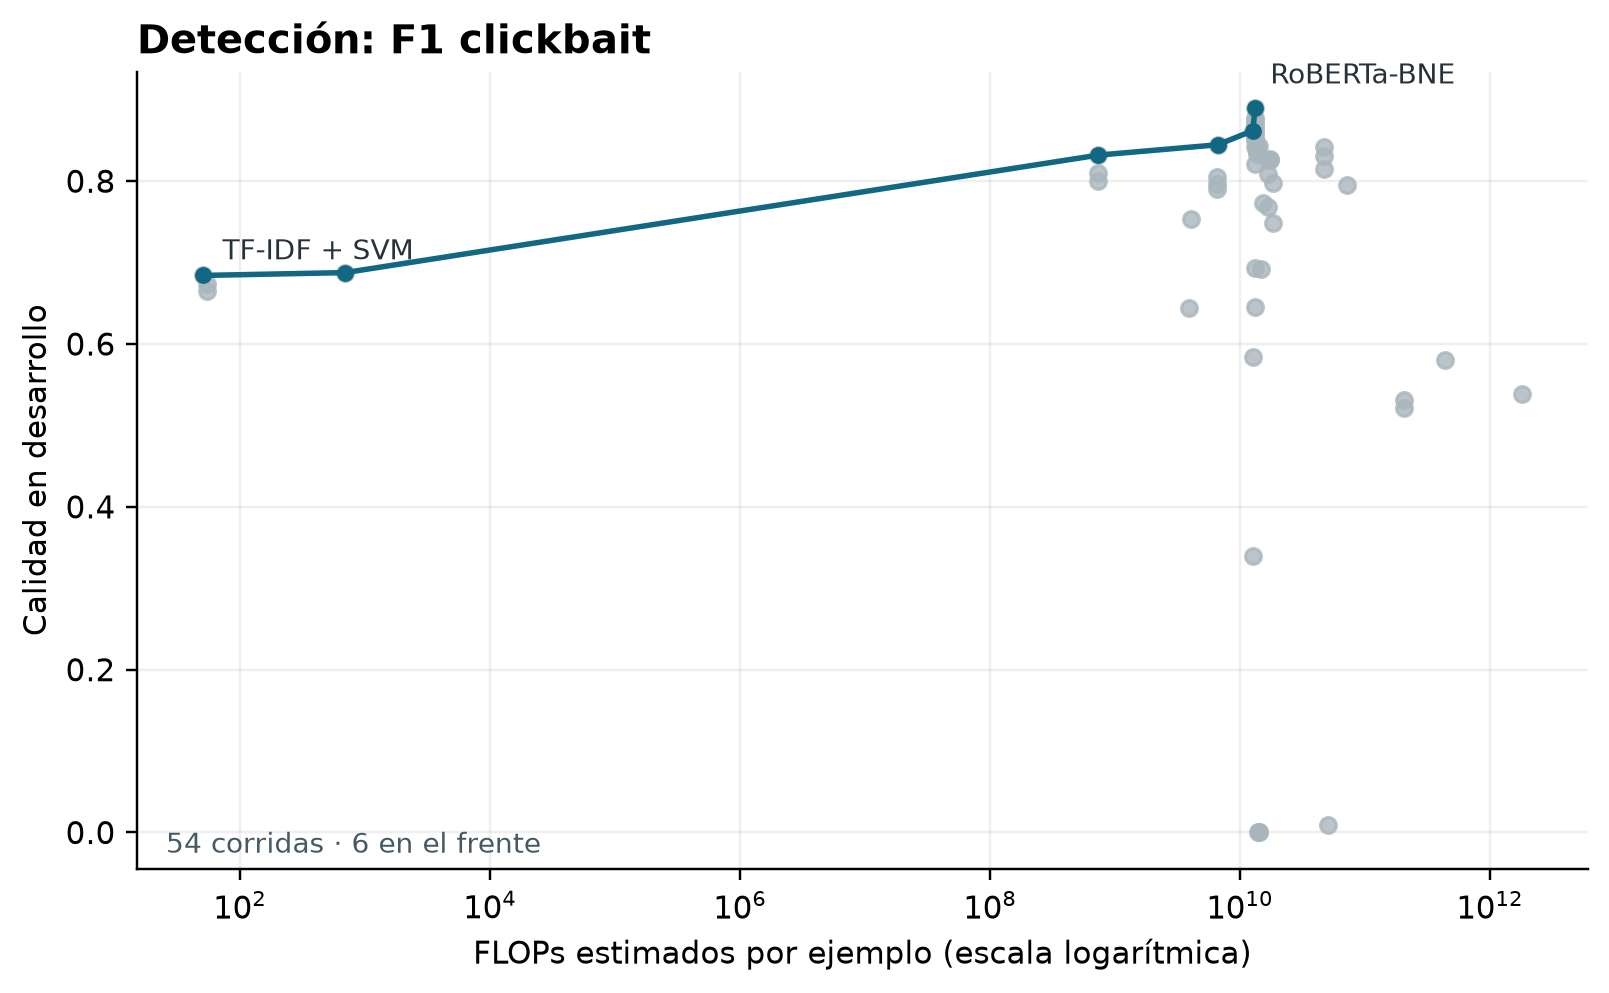
\includegraphics[width=\textwidth]{figuras/frente_detection.png}
\caption{Calidad y cómputo de detección en desarrollo. Los FLOPs se
estiman por ejemplo; la línea une los puntos no dominados.}
\label{fig:pareto-det}
\end{figure}

\begin{figure}[htbp]
\centering
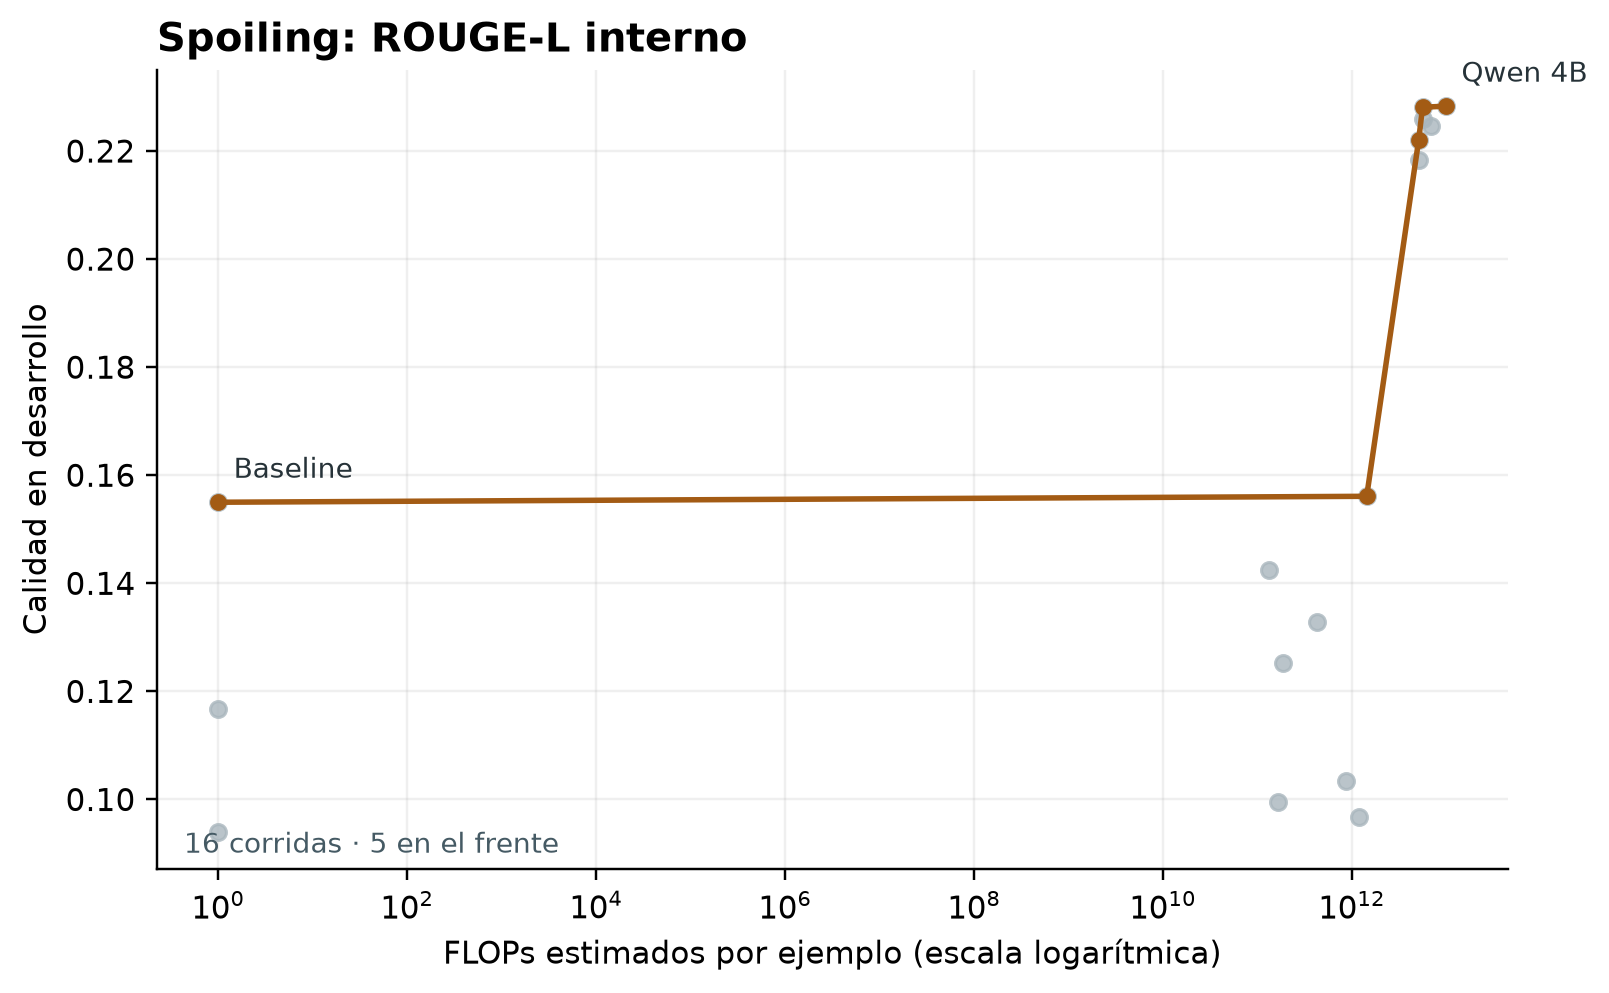
\includegraphics[width=\textwidth]{figuras/frente_spoiling.png}
\caption{Calidad y cómputo de spoiling en desarrollo. ROUGE-L procede de
la implementación local. Los servicios por API no tienen FLOPs comparables.}
\label{fig:pareto-spo}
\end{figure}

\section{Spoiling: calidad interna y salidas}

La réplica de la heurística oficial obtuvo ROUGE-L local 0,1550 y
BERTScore 0,6533 en los 100 ejemplos de desarrollo. En prueba, su BERTScore
fue 0,6637, cercano al 0,661 informado por la tarea compartida. En
desarrollo, Qwen 3.5 4B obtuvo ROUGE-L 0,2283 y BERTScore 0,6996.
GPT-5.6 Luna alcanzó 0,2884 y 0,7273 sin imagen; con imagen, 0,3151
y 0,7350. La diferencia pareada de ROUGE-L fue $+0,0267$, con IC del
95\,\% $[-0,0073;0,0641]$, que incluye cero. Estas corridas generativas
aún no tienen una evaluación final en prueba. En las condiciones de estas
ejecuciones, Luna costó aproximadamente USD 0,327 por 1.000 ejemplos sin
imagen y USD 0,636 con imagen. Ese costo no es comparable con los FLOPs
de los modelos locales.

\section{Aporte de la imagen}

Las figuras~\ref{fig:vision-det} y~\ref{fig:vision-spo} muestran las
comparaciones pareadas entre T y TI. En D10a, DeiT+Beto pasó de F1
0,6960 a 0,6718 al añadir la imagen: una diferencia de $-0,0242$,
con IC del 95\,\% $[-0,0444;-0,0055]$ sobre 3.500 predicciones OOF.
La variante con SigLIP2 también bajó $-0,0254$
($[-0,0499;-0,0002]$). Estos descensos corresponden a las
arquitecturas y entradas probadas.

D10b, con MLP residual, pasó de F1 0,8500 (T) a 0,8523 (TI):
una diferencia de $+0,0023$, con IC del 95\,\% $[-0,0047;0,0098]$.
Las cuatro comparaciones D11, realizadas con una semilla, tampoco
mostraron una mejora concluyente. Las diferencias fueron $+0,0009$ para
MLP \emph{fixed}, $-0,0005$ para atención \emph{fixed}, $-0,0035$ para
MLP \emph{joint} y $+0,0023$ para atención \emph{joint}; todos los
intervalos incluyeron cero. Con \emph{fixed}, las predicciones de los
555 ejemplos sin imagen son idénticas a las del modelo textual. Con
\emph{joint}, el entrenamiento también cambia algunas de esas
predicciones, de modo que la diferencia no refleja solo el uso de la imagen.

En spoiling, las tres comparaciones de Gemma 4 E2B con imagen o pie de
foto tuvieron diferencias de ROUGE-L entre $+0,0026$ y $+0,0061$.
LFM 2.5 VL registró $-0,0067$. Todos los intervalos del 95\,\%
incluyeron cero. En conjunto, estos experimentos no muestran una mejora
visual general en las configuraciones estudiadas y señalan qué casos
merecen una evaluación más controlada.

\begin{figure}[htbp]
\centering
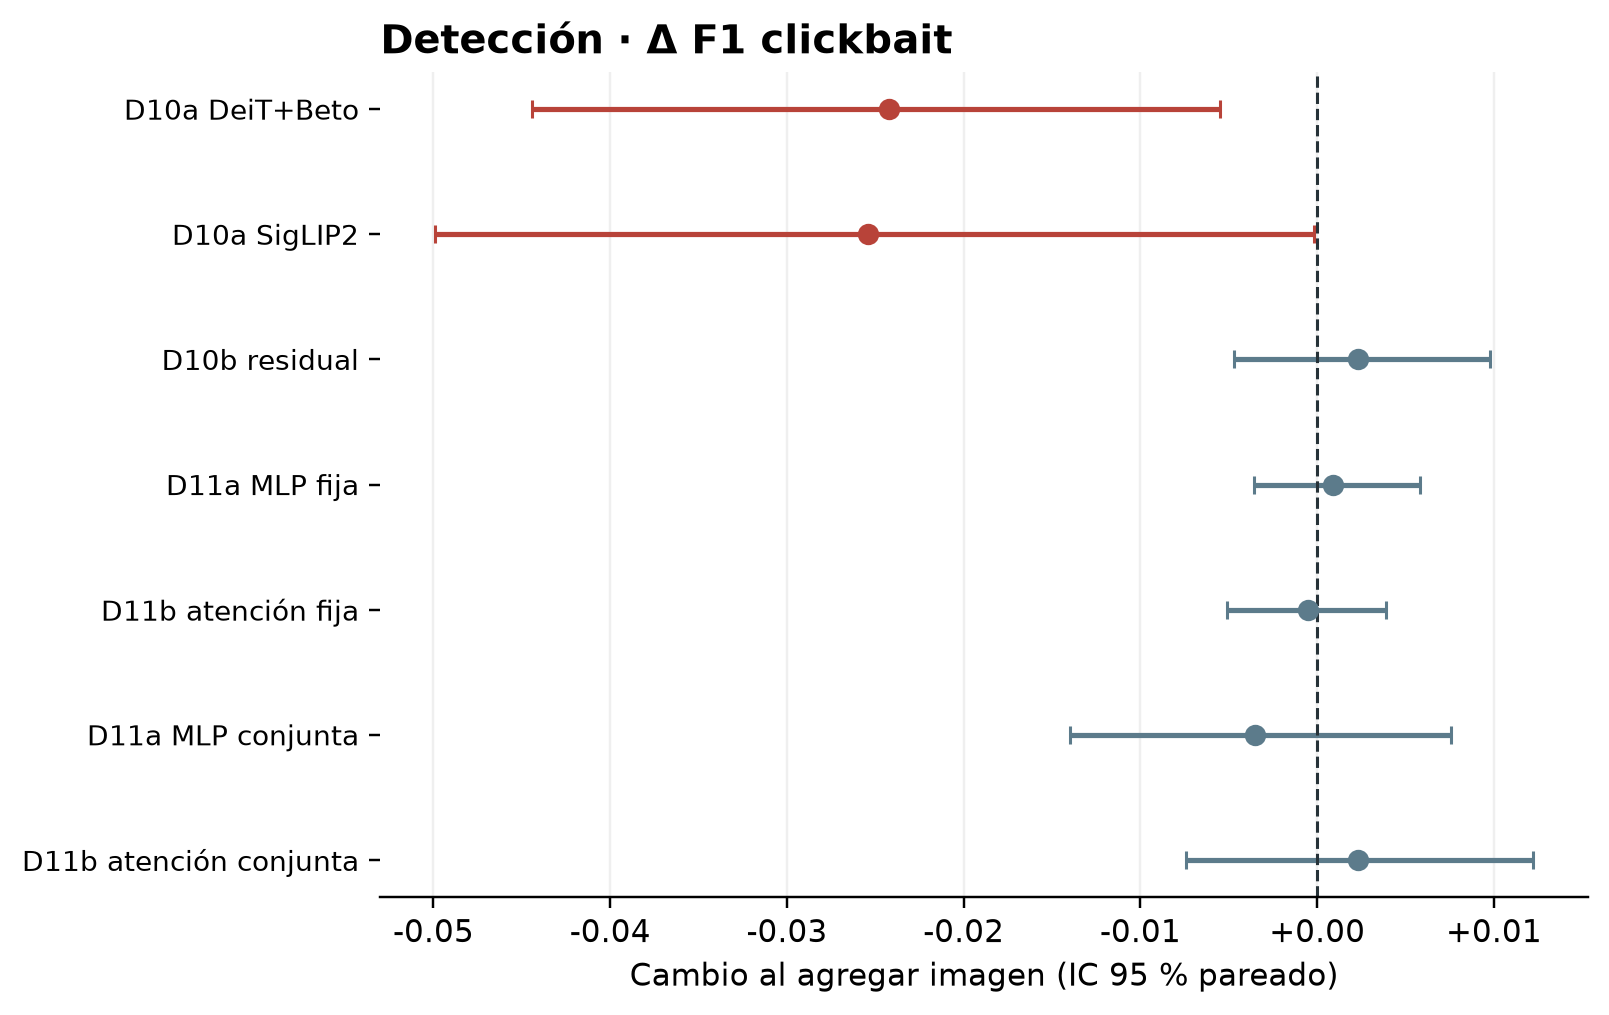
\includegraphics[width=\textwidth]{figuras/ablacion_detection.png}
\caption{Diferencia pareada de F1 al añadir imagen en detección. Se
muestran todos los ejemplos; D10 y D11 usan predicciones OOF.}
\label{fig:vision-det}
\end{figure}

\begin{figure}[htbp]
\centering
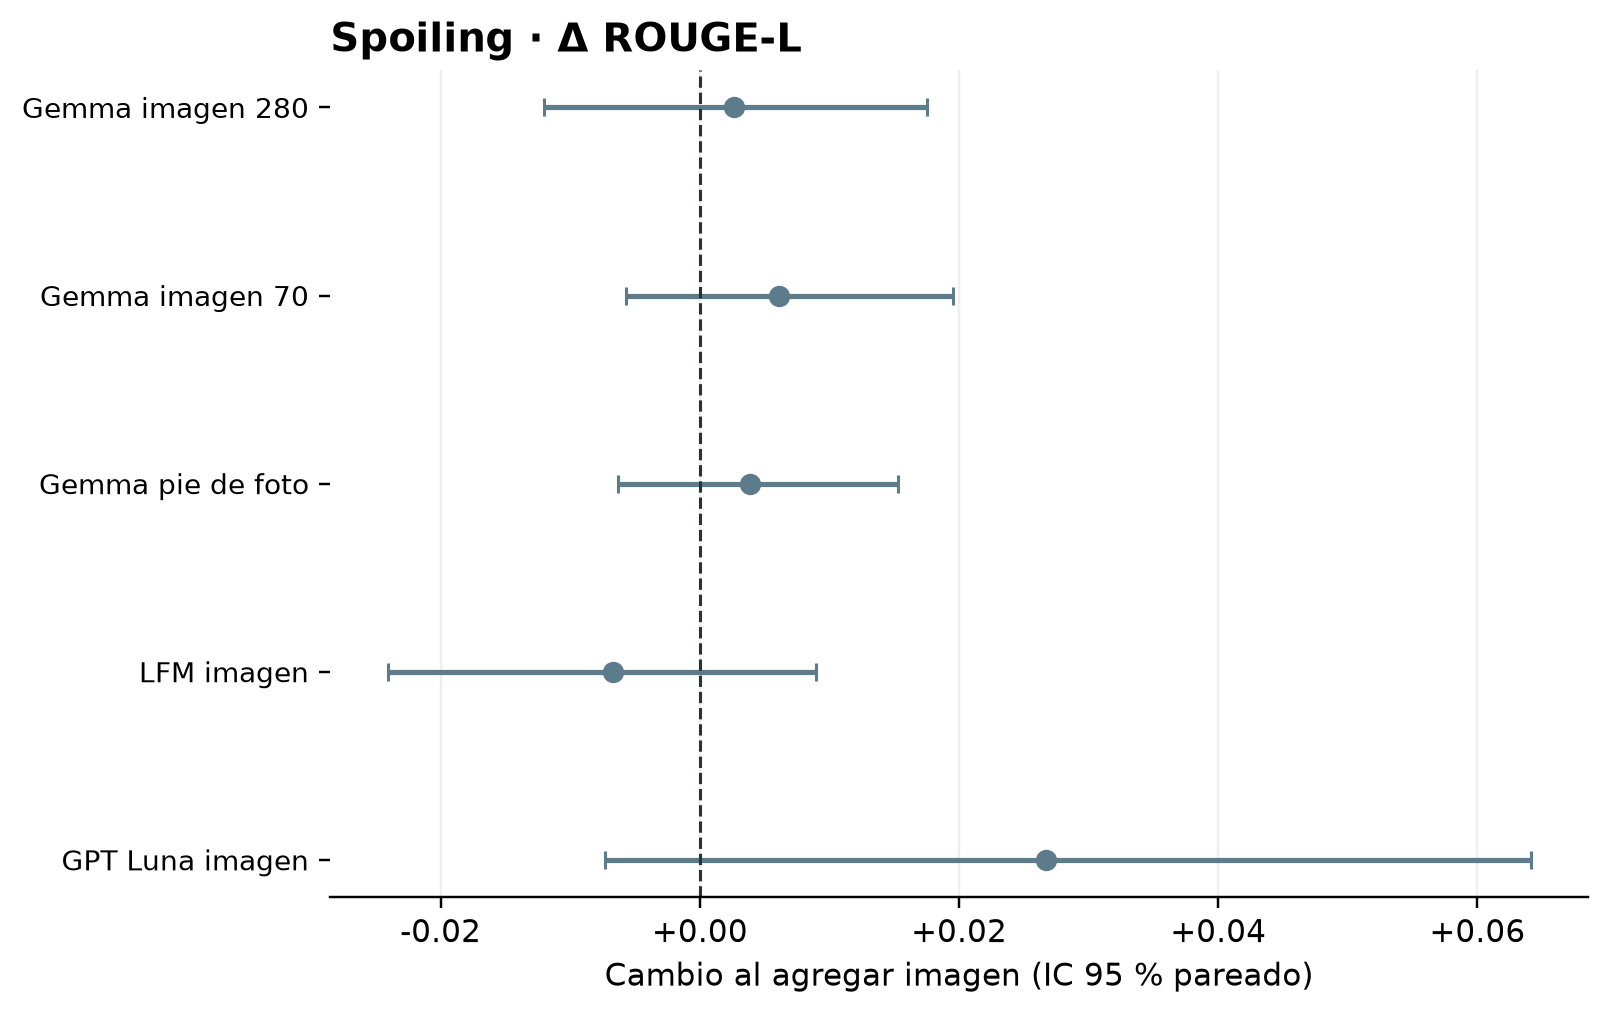
\includegraphics[width=\textwidth]{figuras/ablacion_spoiling.png}
\caption{Diferencia pareada de ROUGE-L local al añadir imagen o pie de
foto en spoiling, sobre todos los ejemplos de desarrollo.}
\label{fig:vision-spo}
\end{figure}

\section{Límites de interpretación}

Varias configuraciones se eligieron según su resultado en desarrollo, por
lo que las mejores cifras de ese conjunto pueden ser optimistas. Además,
la validación visual no separa duplicados, D11 se ejecutó con una sola
semilla y las imágenes recuperadas varían en disponibilidad y pertinencia.
Los intervalos calculados no recogen toda esa incertidumbre ni la selección
de familias de modelos después de inspeccionar desarrollo. El test oficial
de detección carece de imágenes y artículos, de modo que no es una prueba
final de los modelos multimodales. Las versiones
locales de ROUGE-L y BLEU tampoco reproducen la evaluación oficial de
spoiling. Por último, la comparación entre calidad y costo no incluye
la obtención de imágenes, el tiempo total de respuesta ni la valoración
humana de los spoilers. Los resultados deben leerse con estos límites
al establecer referencias para evaluar el marco de agentes.

\chapter[Evaluación y transferencia]{Protocolo de evaluación del marco y transferencia}
\label{cap:evaluacion-marco}

La evaluación del marco debe distinguir la calidad de una solución individual de la eficacia del proceso que la encontró. Los resultados del estudio de base establecen referencias y riesgos metodológicos, pero no permiten atribuir mejoras a los agentes. La comparación principal se realiza entre estrategias de búsqueda que disponen de los mismos datos, espacio de soluciones y límites de recursos.

\section{Comparadores y presupuesto}

La referencia mínima es una búsqueda aleatoria reproducible sobre el mismo espacio de candidatos; una grilla pequeña o una selección manual documentada pueden ampliar la comparación. La búsqueda aleatoria es una referencia establecida para optimización de hiperparámetros \citep{bergstra2012}. Antes de ejecutar las estrategias se fijan el número máximo de intentos, el tiempo de cómputo, las consultas a servicios externos y sus costos. Se registran los valores efectivos de esos recursos, incluidos los intentos que fallan o exceden el tiempo. Si una estrategia consume menos que su límite, se informa el recurso no utilizado.

Para cada estrategia se traza la mejor calidad válida encontrada frente al costo acumulado. Además de la puntuación final se informa el área bajo esa trayectoria o un resumen equivalente, la variación entre semillas, la proporción de candidatos válidos y el tiempo necesario para reproducir el mejor resultado. La selección se hace en desarrollo o validación cruzada; la partición final se consulta una vez después de congelar la configuración elegida.

\section{Detección y generación de clickbait}

En detección se conservan las particiones y la definición de la clase positiva de TA1C. Las familias comparadas reciben las mismas entradas, y las configuraciones que usan imagen se analizan aparte porque el test oficial carece de esa modalidad. El informe incluye F1 de clickbait, F1 macro, precisión, exhaustividad y matrices de confusión, con intervalos pareados para diferencias entre estrategias sobre los mismos casos. Los duplicados de noticia, evento o imagen deben identificarse antes de cerrar la partición final.

En \emph{spoiling}, la búsqueda usa una métrica automática cuya implementación queda fijada junto con las restricciones de longitud. La evaluación final añade un juicio humano sobre si la respuesta está sustentada en el artículo, responde a la pregunta, es concisa y se entiende sin el enlace. La muestra y la rúbrica se fijan antes de inspeccionar las salidas; se informa el acuerdo entre evaluadores y se revisan desacuerdos. Las referencias humanas de TA1C que exceden el límite de 280 caracteres se analizan como una fuente de sesgo de las métricas de solapamiento.

\section{Ablaciones del proceso de agentes}

Para atribuir efectos a los componentes del marco se comparan, con el mismo presupuesto, el ciclo completo y variantes que eliminan o sustituyen una función. El proponente puede reemplazarse por muestreo aleatorio; el analista puede recibir solo la última corrida en lugar del historial; y el ejecutor puede conservar las mismas comprobaciones deterministas mientras se desactiva la reparación automática de fallos. Cada variante mantiene los mismos datos y reglas de validez. La interpretación debe separar diferencias de calidad de diferencias en número de candidatos ejecutados correctamente.

\section{Transferencia a otra tarea}

La prueba de transferencia utiliza una tarea textual distinta del clickbait. La detección de fraude en mensajes, como phishing o estafas, es una opción si se dispone de un corpus con licencia, etiquetas y partición adecuadas. Antes de ejecutarla se documentan los cambios exigidos por la nueva tarea: adaptador de datos, espacio de candidatos, métrica, verificaciones, prompts y recursos. La lógica del ciclo y el formato del registro permanecen como objetos de evaluación: cualquier modificación de ellos se informa como límite de la reutilización.

La transferencia se juzga con dos medidas complementarias. La primera es el desempeño frente a una referencia propia de la nueva tarea bajo el mismo presupuesto. La segunda es el esfuerzo de adaptación, medido mediante componentes modificados, tiempo de implementación y fallos de integración. Un resultado favorable en un dominio adicional respalda una portabilidad delimitada; no basta para afirmar que el marco es útil en cualquier tarea de PLN.

% Incorporar aquí, cuando existan, tablas de resultados del marco con:
% tarea, estrategia, presupuesto planificado y consumido, semillas,
% calidad en validación y prueba, tasa de fallos, costo, intervalos y
% análisis de errores. Registrar también el corpus y resultado de transferencia.

% \chapter{Resultados del marco de agentes}
\label{cap:resultados-marco}

% Activar este capítulo en main.tex cuando existan corridas del marco.
% En cada tabla: tarea, estrategia, espacio de candidatos, semillas,
% presupuesto planificado y efectivo, calidad en desarrollo y prueba,
% candidatos válidos/fallidos, costo total e intervalo de incertidumbre.

\section{Detección de clickbait}
% Comparar trayectorias de búsqueda y mejores candidatos con referencias.

\section{Generación de spoilers}
% Informar métrica automática, evaluación humana y análisis de errores.

\section{Ablaciones del ciclo de agentes}
% Aislar propuesta, ejecución verificada, análisis y memoria.

\section{Transferencia a otra tarea}
% Describir corpus, adaptaciones, desempeño y esfuerzo de adaptación.

\section{Síntesis y amenazas a la validez}
% Responder qué generaliza y qué depende de tarea, datos o presupuesto.
 % Activar tras incorporar resultados del marco.
% % Capítulo pendiente. Redactar conclusiones cuando existan resultados de la
% comparación del ciclo de agentes, de calidad y costo, y de la auditoría de datos.
% Activar su entrada en main.tex después de responder las preguntas de investigación.
 % Redactar cuando exista evidencia para responder las preguntas de investigación.

\backmatter
\bibliographystyle{plainnat}
\bibliography{referencias}

\end{document}
